\section{Formalizing the Bipartisan Paxos Protocols}\seclabel{FormalBPaxosOverview}
The BPaxos protocols implement state machine replication. Informally, a set of
client processes repeatedly propose state machine commands, and a set of state
machine replicas all execute the commands in exactly the same order (modulo the
reordering of non-conflicting commands). In this section, we formalize state
machine replication by way of generalized consensus and then overview the
common structure that underlies all of the BPaxos protocols. But first, we take
a brief detour through some mathematical preliminaries.

\subsection{BPaxos Graphs and Partial BPaxos Graphs}
Consider a set $\Cmd$ of commands and a symmetric conflict relation
$\conflict$. A \defword{BPaxos graph} (with respect to $\Cmd$ and $\conflict$)
is a directed (potentially cyclic) graph $B = (V, E, \varphi)$ where
%
  $V$ is a set of vertices;
%
  $E \subseteq V \times V$ is a set of edges;
%
  $\varphi: V \to \Cmd$ is a function that labels every vertex with a command;
  and
%
  for every pair of vertices $v_1, v_2 \in V$, there exists an edge between
  $v_1$ and $v_2$ if (but not only if) $\varphi(v_1)$ and $\varphi(v_2)$
  conflict.
%
Intuitively, a BPaxos graph is a potentially cyclic conflict graph (see
\secref{ConflictGraphs}) that can have spurious edges between vertices labelled
with non-conflicting commands.

A \defword{partial BPaxos graph} $B = (V, E, \varphi)$ is a BPaxos graph except
that $\varphi: V \partialto \Cmd$ is partial. Intuitively, a partial BPaxos
graph is a BPaxos graph for which the labels of some vertices are unknown.
%
We say a vertex $v$ in a partial BPaxos graph is \defword{eligible} if $v$ and
all vertices reachable from $v$ are labelled. The \defword{eligible suffix} of
a partial BPaxos graph $B$ is the suffix of $B$ consisting of all eligible
vertices.
%
An example partial BPaxos graph is illustrated in \figref{PartialBPaxosGraph},
and its eligible suffix is shown in \figref{EligibleSuffix}.

\begin{figure}[ht]
  \centering
  \tikzstyle{vertex}=[draw, minimum width=16pt, minimum height=16pt]
  \tikzstyle{arrow}=[thick, -latex]

  \begin{subfigure}[b]{2in}
    \centering
    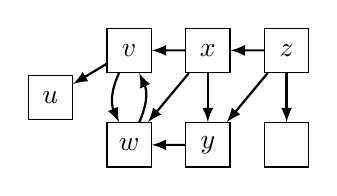
\begin{tikzpicture}[xscale=1, yscale=0.6]
      \node[vertex] (u) at (0, 0) {$u$};
      \node[vertex] (v) at (1, 1) {$v$};
      \node[vertex] (w) at (1, -1) {$w$};
      \node[vertex] (x) at (2, 1) {$x$};
      \node[vertex] (y) at (2, -1) {$y$};
      \node[vertex] (z) at (3, 1) {$z$};
      \node[vertex] (unknown) at (3, -1) {\phantom{z}};

      \draw[arrow] (v) to (u);
      \draw[arrow, bend right=15] (v) to (w);
      \draw[arrow, bend right=15] (w) to (v);
      \draw[arrow] (x) to (v);
      \draw[arrow] (x) to (w);
      \draw[arrow] (x) to (y);
      \draw[arrow] (y) to (w);
      \draw[arrow] (z) to (x);
      \draw[arrow] (z) to (y);
      \draw[arrow] (z) to (unknown);
    \end{tikzpicture}
    \caption{A partial BPaxos graph $B$}\figlabel{PartialBPaxosGraph}
  \end{subfigure}%
  \begin{subfigure}[b]{2in}
    \centering
    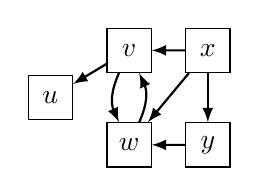
\begin{tikzpicture}[xscale=1, yscale=0.6]
      \node[vertex] (u) at (0, 0) {$u$};
      \node[vertex] (v) at (1, 1) {$v$};
      \node[vertex] (w) at (1, -1) {$w$};
      \node[vertex] (x) at (2, 1) {$x$};
      \node[vertex] (y) at (2, -1) {$y$};

      \draw[arrow] (v) to (u);
      \draw[arrow, bend right=15] (v) to (w);
      \draw[arrow, bend right=15] (w) to (v);
      \draw[arrow] (x) to (v);
      \draw[arrow] (x) to (w);
      \draw[arrow] (x) to (y);
      \draw[arrow] (y) to (w);
    \end{tikzpicture}
    \caption{The eligibile suffix $B'$ of $B$}\figlabel{EligibleSuffix}
  \end{subfigure}%
  \begin{subfigure}[b]{2in}
    \centering
    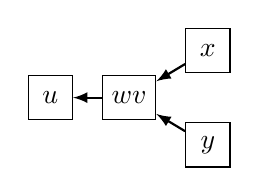
\begin{tikzpicture}[xscale=1, yscale=0.6]
      \node[vertex] (u) at (0, 0) {$u$};
      \node[vertex] (vw) at (1, 0) {$wv$};
      \node[vertex] (x) at (2, 1) {$x$};
      \node[vertex] (y) at (2, -1) {$y$};

      \draw[arrow] (vw) to (u);
      \draw[arrow] (x) to (vw);
      \draw[arrow] (y) to (vw);
    \end{tikzpicture}
    \caption{The condensation of $B'$}\figlabel{Condensation}
  \end{subfigure}

  \caption{}
\end{figure}


The \defword{condensation} of BPaxos graph $B$ is the graph obtained by first
removing spurious edges between non-conflicting vertices in $B$ and then by
contracting every strongly connected component. Every strongly connected
component labelled with commands $x_1, \ldots, x_n$ is replaced with a single
vertex labelled with a command string $x_{i_1} x_{i_2} \cdots x_{i_n}$ that is
obtained from an arbitrary but fixed ordering of the commands $x_1, \ldots,
x_n$. An example condensation is shown in \figref{Condensation}.
%
The condensation of a BPaxos graph with respect to $\Cmd$ and $\conflict$ is
a conflict graph with respect to $\Cmd^+$ and $\conflict^+$ where $\Cmd^+$ is
the set of non-empty command strings and where $(x_1 x_2 \cdots x_n, y_1 y_2
\cdots y_m) \in \conflict^+$ if there is some $x_i$ and $y_j$ that conflict in
$\conflict$.

\subsection{Problem Description}
The BPaxos protocols implement state machine replication by way of generalized
consensus. We assume an asynchronous network model and deterministic processes
that can fail by crashing (but cannot act maliciously). Throughout the paper,
we assume at most $f$ processes can fail.  We consider a set $b_1, b_2, \ldots,
b_{f+1}$ of deterministic state machine replicas that all begin in the same
initial state. We consider a set $\Cmd$ of state machine commands and define a
conflict relation $\conflict$ such that two commands $x, y \in \Cmd$ conflict
if they do not commute--i.e.\ if there exists a state in which executing $x$
and then $y$ does not produce the same responses and final state as executing
$y$ and then $x$.

Every BPaxos protocol is a generalized consensus protocol (see
\secref{GeneralizedConsensus}), with state machine replicas playing the role of
learners. Each replica $b_i$ learns a conflict graph $C_i$ with respect to
$\Cmd^+$ and $\conflict^+$. Every replica $b_i$ executes the commands in $C_i$
in reverse topological order as they are learned. For example, if a replica has
learned the conflict graph shown in \figref{Condensation}, it can execute
commands in the order $uwvxy$ or $uwvyx$.  Executing commands in this way,
replicas are guaranteed to stay in sync, producing identical responses for
every command they execute.

\subsection{BPaxos Protocols Overview}
Every BPaxos protocol implements generalized consensus by first reaching
consensus on a partial BPaxos graph.
%
When a client process sends a state machine command $x$ to a BPaxos protocol, a
process implementing the protocol eventually assigns the command an identifier
$I$ called an \defword{instance} and a set of instances, $\deps{I}$, called the
\defword{dependencies} of $I$.
%
The BPaxos protocol implements one instance of consensus for every instance $I$
and eventually reaches consensus on the value $(x, \deps{I})$ in instance $I$.
Every state machine replica $b_i$ maintains a partial BPaxos graph $B_i$ where
instances play the role of vertices. When replica $b_i$ learns that an instance
$I$ has been chosen with value ($x$, $\deps{I}$), it adds vertex $I$ to $B_i$
labelled with $x$ and with outbound edges to every instance in $\deps{I}$
(adding previously unseen instances to $B_i$ as necessary). Letting $C_i$ be
the condensation of the eligible suffix of $B_i$, the BPaxos protocol
successfully implements generalized consensus with replica $b_i$ learning
conflict graph $C_i$ so long as the following two invariants are met.

\begin{invariant}\invlabel{ConsensusInvariant}
  The BPaxos protocol successfully implements consensus for every instance $I$.
  That is, at most one value $(x, \deps{I})$ is chosen in instance $I$ (i.e.\
  consistency), and if the value $(x, \deps{I})$ is chosen, then it was
  previously proposed (i.e.\ nontriviality).
\end{invariant}%
%
\begin{invariant}\invlabel{ConflictInvariant}
  If $(x, \deps{I_x})$ is chosen in instance $I_x$ and $(y, \deps{I_y})$ is
  chosen in instance $I_y$, and if $x$ and $y$ conflict, then either $I_x \in
  \deps{I_y}$ or $I_y \in \deps{I_x}$ or both.
\end{invariant}

\invref{ConsensusInvariant} allows replicas to reach consensus on their partial
BPaxos graphs. \invref{ConflictInvariant} ensures that every replica's partial
BPaxos graph really is a partial BPaxos graph. These two invariants suffice to
ensure stability and consistency (see \secref{GeneralizedConsensus}).
%
Stability is guaranteed because a replica $b_i$'s partial BPaxos graph $B_i$
(and hence its condensation $C_i$) only grows over time.
%
Consistency is guaranteed because every condensation $C_i$ is a prefix of the
condensation of the eligible suffix of the global partial BPaxos graph, the
graph formed from complete knowledge of every chosen instance.
%
The BPaxos protocols do provide liveness with certain assumptions about the
niceness of the network, but we do not focus on liveness in this paper.
%
Finally, every BPaxos protocol ensures nontriviality in a straightforward way.

Every BPaxos protocol follows this pattern of reaching consensus on a partial
BPaxos graph one instance at a time and locally computing condensations of
eligible suffixes. The protocols differ only in how they compute dependencies
and how they reach consensus for a given instance. Thus, to prove the
safety of a BPaxos protocol, it suffices to prove that the protocol maintains
\invref{ConsensusInvariant} and \invref{ConflictInvariant}.
